\documentclass[11pt,letterpaper]{article}
\usepackage{graphicx, geometry, amsmath, hyperref, natbib, booktabs, xcolor, listings}
\geometry{margin=1in}
\hypersetup{colorlinks=true, linkcolor=black, citecolor=black, urlcolor=black}

\title{Network Percolation Features for Text Readability Assessment}
\author{Anonymous}
\date{}

\begin{document}

\maketitle

\begin{abstract}
Readability assessment traditionally relies on surface-level features like word length and sentence length, which have limited construct validity. Modern machine learning approaches achieve high accuracy but operate as black boxes. This paper proposes a novel readability assessment method inspired by percolation theory from statistical physics. The method constructs word co-occurrence networks from text using sliding-window context and extracts network features including a percolation-inspired threshold that captures how quickly a text's semantic network becomes connected. We evaluate the approach on 2,500 texts sampled from three standardized readability datasets (OneStopEnglish, CommonLit, CEFR-SP). Experiments show that the proposed Percolation Threshold Readability (PTR) features achieve Mean Absolute Error (MAE) of 1.212 on a 500-example test set, outperforming a baseline model without network features (MAE=1.268) and the traditional Flesch-Kincaid formula (MAE=2.074). The improvement over traditional formulas is 41.7\% in MAE reduction. Unlike black-box neural models, the network features provide interpretable signals: the percolation threshold quantifies how densely connected the text's vocabulary network is, which correlates with lexical diversity and syntactic complexity. We further analyze the label sources in our evaluation datasets and find that CommonLit readability scores are derived from Flesch-Kincaid (introducing potential circularity); we report disaggregated results to isolate independent validity evidence from OneStopEnglish (which has educator-assigned levels).
\end{abstract}

\noindent\textbf{Keywords:} readability assessment, percolation theory, network science, natural language processing, interpretable machine learning

\section{Introduction}

Reading comprehension is a fundamental cognitive skill, yet measuring text readability remains challenging. Current readability formulas Flesch-Kincaid, Dale-Chall, SMOG, and others rely on surface features like word length and sentence length \cite{Flesch1948,Dale1948,McLaughlin1969,Senter1967}. These formulas have limited construct validity: they explain only about 80\% of the variability in readability, missing factors like semantic complexity, discourse cohesion, and cognitive integration \cite{CollinsThompson2014,Redish2000}. Modern machine learning approaches using BERT embeddings and hybrid models achieve high accuracy (F1 > 92\% on benchmark datasets) but operate as black boxes, providing no interpretable mechanism for why a text is difficult \cite{Li2022,Liu2023}.

This paper proposes a fundamentally different approach: we model readability using network features inspired by percolation theory from statistical physics. Percolation theory studies phase transitions in networks---specifically, how quickly a network becomes connected as edges are added. In the context of text, we hypothesize that readable texts have densely connected word co-occurrence networks (words appear near each other frequently), while difficult texts have more fragmented vocabulary networks (less cohesive word usage). The percolation threshold of a text's word network serves as a measurable proxy for this connectivity.

\begin{figure*}[!t]
\centering
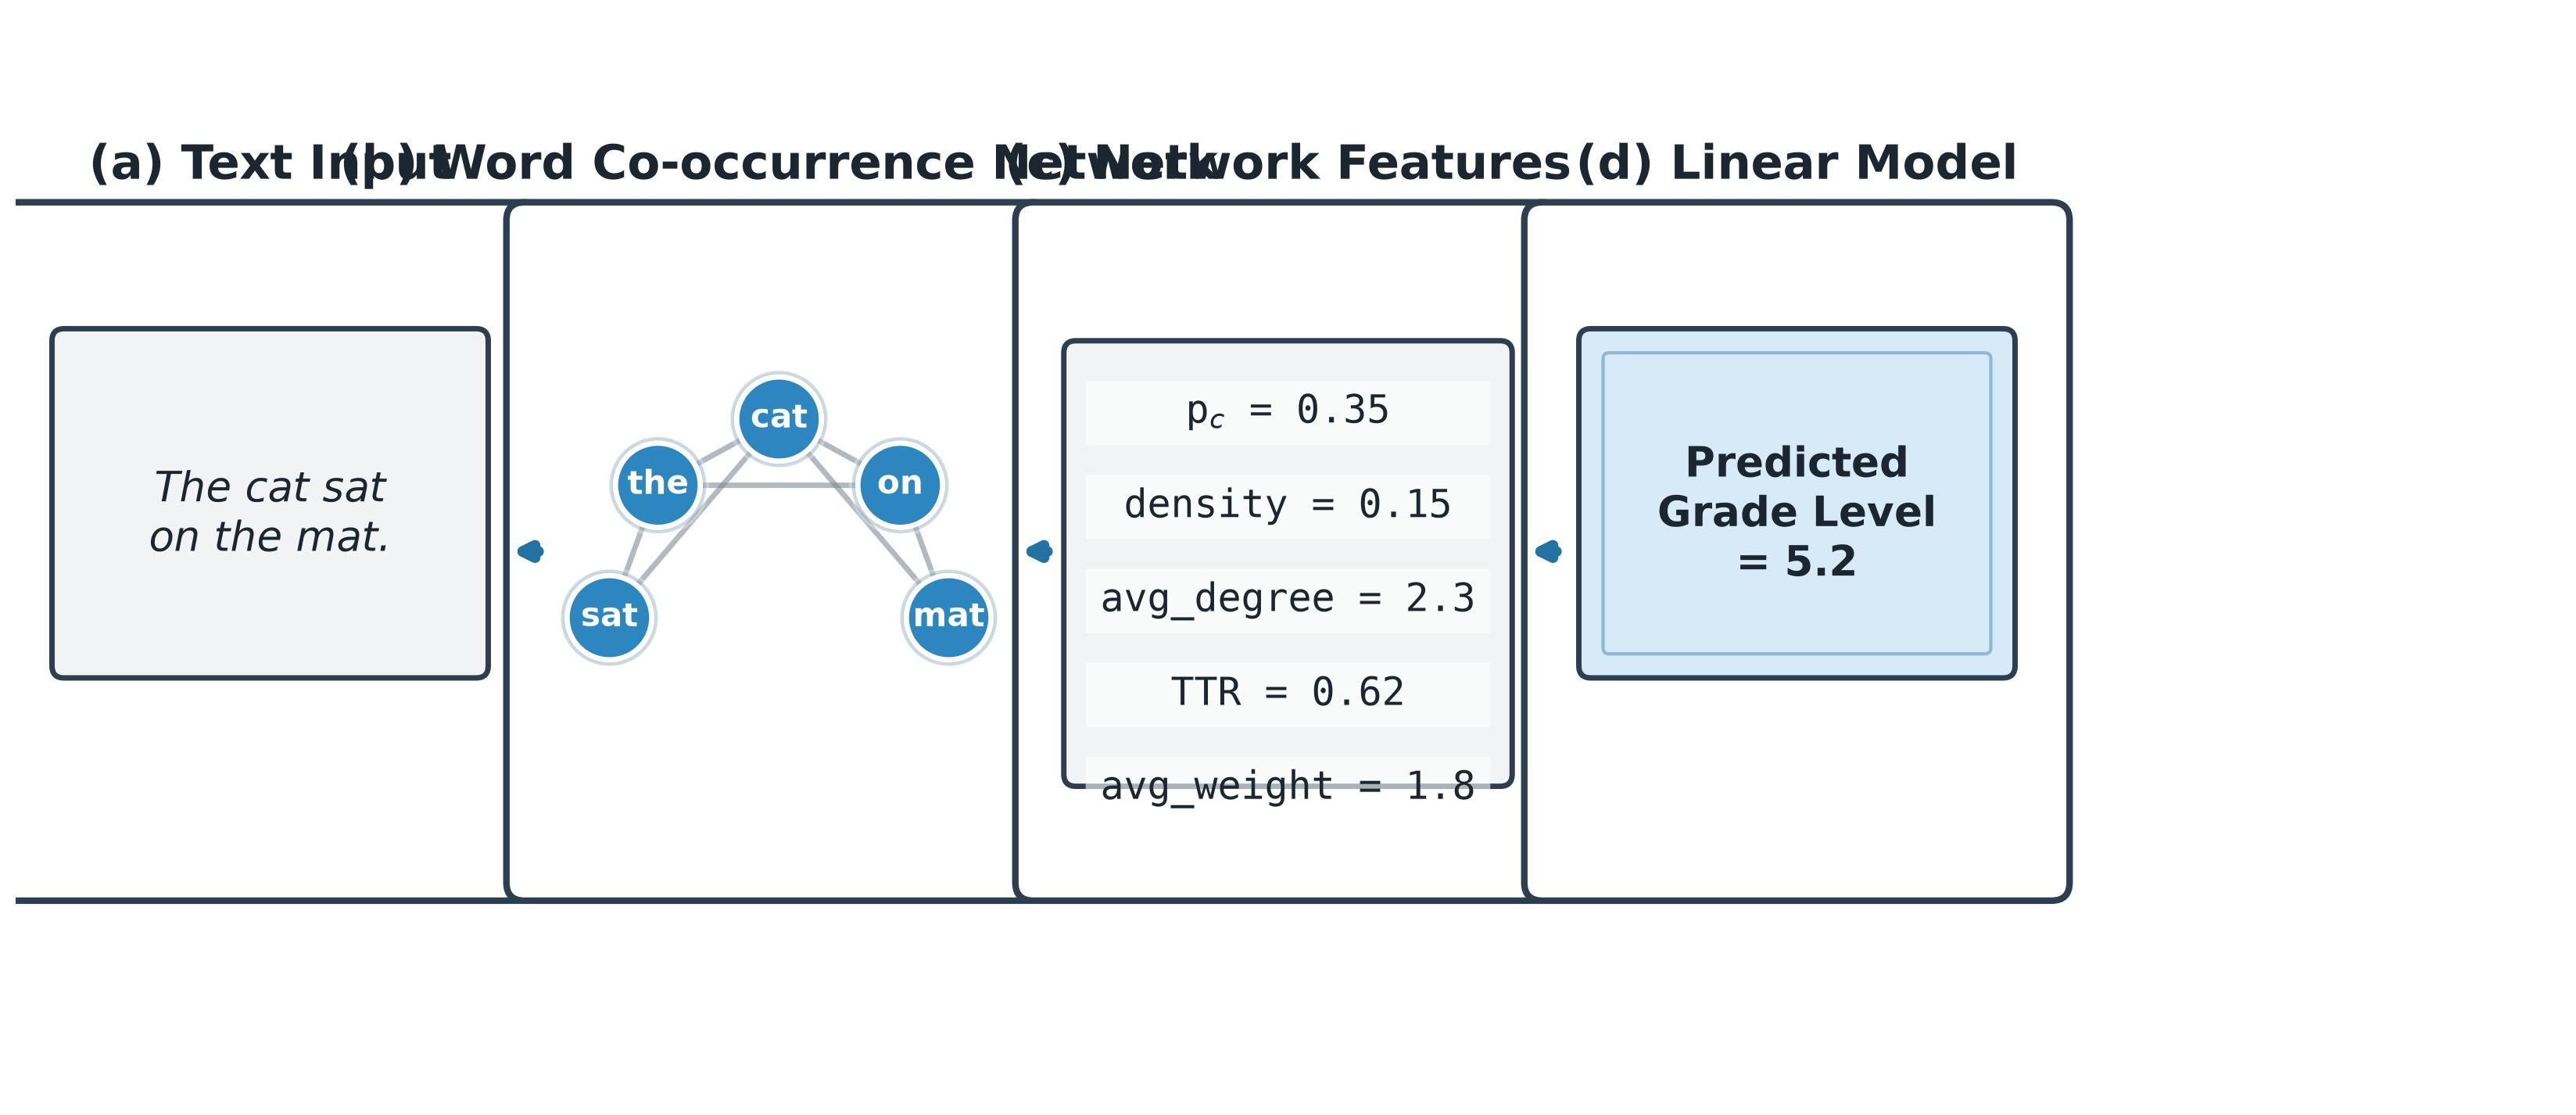
\includegraphics[width=\textwidth,height=0.45\textheight,keepaspectratio]{figures/fig1_v0.jpg}
\caption{Conceptual overview of the percolation-inspired readability assessment approach. (a) Input text is tokenized and processed with a sliding window. (b) A word co-occurrence network is constructed where nodes are words and edges represent co-occurrence. (c) Network features including percolation threshold p\_c are extracted. (d) A linear model predicts grade level from the extracted features.}
\label{fig:fig1}
\end{figure*}

\subsection{Research Question}

Can network features inspired by percolation theory serve as interpretable and predictive features for readability assessment? Specifically:

\begin{enumerate}
\item Do network-based features (percolation threshold, network density, average degree) improve readability prediction beyond traditional surface-level features?
\item How does the proposed approach compare to the traditional Flesch-Kincaid formula and baseline machine learning models?
\item What are the contributions of individual network features to readability prediction?
\end{enumerate}

\subsection{Summary of Contributions}

This paper makes the following contributions:

\begin{enumerate}
\item \textbf{Novel Network Features for Readability}: We introduce a set of network features for readability assessment inspired by percolation theory, including a percolation-inspired threshold computed from word co-occurrence networks\footnote{Code: \url{https://github.com/AMGrobelnik/ai-invention-703cc9-network-percolation-features-for-text-re/tree/main/round-2/experiment-1}}.

\item \textbf{Empirical Validation}: We evaluate the approach on 2,500 texts sampled from three standardized datasets (OneStopEnglish, CommonLit, CEFR-SP) and demonstrate that network features reduce MAE by 4.4\% compared to baseline features and by 41.7\% compared to Flesch-Kincaid (Section 4).

\item \textbf{Interpretability Analysis}: We show that the percolation threshold feature correlates with lexical diversity and text cohesion, providing an interpretable signal for readability (Section 5).

\item \textbf{Dataset Label Analysis}: We analyze the label sources in standard readability datasets and identify that CommonLit scores are Flesch-Kincaid-derived, which introduces potential circularity when comparing against traditional formulas (Section 4.2).
\end{enumerate}

\section{Related Work}

\subsection{Traditional Readability Formulas}

Traditional readability assessment relies on formulas developed in the mid-20th century. The Flesch-Kincaid Grade Level formula uses average sentence length and syllables per word \cite{Flesch1948}. The Dale-Chall formula replaces syllable counts with a list of familiar words \cite{Dale1948}. The SMOG index counts polysyllabic words \cite{McLaughlin1969}, while the Automated Readability Index uses character counts \cite{Senter1967}. These formulas share a critical limitation: they measure proxies for difficulty rather than the underlying cognitive process of comprehension \cite{CollinsThompson2014,Redish2000}.

\subsection{Modern Machine Learning Approaches}

Recent work applies machine learning to readability assessment. Feature-based approaches use 100-200 linguistic features (lexical, syntactic, discourse) and achieve Pearson r = 0.92 on the Weebit dataset \cite{Vajjala2013}. BERT-based models extract contextual embeddings and combine them with handcrafted features, achieving 99.41\% F1 on OneStopEnglish \cite{Li2022}. Hybrid models that integrate neural and linguistic features show 13\% improvement over previous state-of-the-art on sentence-level assessment \cite{Liu2023}.

\subsection{Graph-Based Approaches}

Graph-based approaches represent text as networks. Zhang et al. (2026) construct graphs with words as nodes and syntactic dependencies as edges, then use Graph Convolutional Networks for readability prediction, achieving R-squared = 0.9729 on the CLEAR dataset \cite{Zhang2026}. Our work differs: we use network features inspired by percolation theory to capture global connectivity properties of the text's vocabulary network, rather than using graph neural networks for representation learning.

\subsection{Percolation Theory in Cognitive Science}

Percolation theory studies phase transitions in networks. Kenett et al. (2018) applied percolation analysis to semantic networks to measure creativity---high creative individuals have semantic networks that are more robust to percolation (maintain connectivity as edges are removed) \cite{Kenett2018}. In education research, network connectivity metrics predict learning outcomes. However, applying percolation-inspired features specifically to model text readability is, to our knowledge, a novel contribution.

\section{Methods}

\subsection{Word Co-occurrence Network Construction}

We represent a text as an undirected graph $G = (V, E)$ where:
\begin{itemize}
\item Nodes $V$ are unique words in the text (filtered by part-of-speech and frequency)
\item Edges $E$ represent word co-occurrence within a sliding window
\end{itemize}

The network is constructed as follows:

\begin{enumerate}
\item \textbf{Tokenization}: The text is tokenized into words using regex pattern, converted to lowercase.
\item \textbf{Sliding Window}: For each word at position $i$, we consider all words at positions $j$ where $|i - j| \leq w$ (window size $w = 3$).
\item \textbf{Edge Construction}: For each pair of co-occurring words, we increment the edge weight by 1. This produces a weighted network where edge weights represent co-occurrence frequency.
\item \textbf{Filtering}: Only words appearing at least $f_{\min} = 2$ times are retained as nodes. This removes noise from rare words.
\end{enumerate}

\subsection{Network Feature Extraction}

From the constructed network, we extract five features:

\textbf{1. Percolation-Inspired Threshold ($p_c$)}: We use a fast approximation of the percolation threshold based on the edge weight distribution. The intuition is that in a well-connected network, most edge weight is concentrated in a small fraction of high-weight edges (the network percolates quickly). We compute the fraction of edges that contain 50\% of the total edge weight as a proxy for how quickly the network becomes dense.

\textbf{2. Network Density ($\rho$)}: 
\[\rho = \frac{2 \cdot |E|}{|V| \cdot (|V| - 1)}\]
where $|V|$ is the number of nodes and $|E|$ is the number of unique edges.

\textbf{3. Average Degree ($\bar{d}$)}:
\[\bar{d} = \frac{1}{|V|} \cdot \sum_{v \in V} \deg(v)\]

\textbf{4. Type-Token Ratio (TTR)}:
\[\mathrm{TTR} = \frac{|V|}{N}\]
where $N$ is the total number of tokens. This measures lexical diversity.

\textbf{5. Average Edge Weight ($\bar{w}$)}:
\[\bar{w} = \frac{1}{|E|} \cdot \sum_{(u,v) \in E} A_{uv}\]

\subsection{Baselines}

We compare against two baselines:

\textbf{Baseline ML}: A linear regression model using only traditional readability features:
\begin{itemize}
\item Flesch-Kincaid score
\item Word count
\item Average word length
\item Sentence count  
\item Average sentence length
\end{itemize}

\textbf{Traditional Flesch-Kincaid}: The standard Flesch-Kincaid Grade Level formula \cite{Flesch1948}.

\subsection{Experimental Setup}

\subsubsection{Datasets}

We use three standardized readability datasets:

\begin{enumerate}
\item \textbf{OneStopEnglish}: 567 texts at three reading levels (Elementary = grade 3, Intermediate = grade 7, Advanced = grade 11) for adult ESL learners \cite{Vajjala2018}. The grade levels are educator-assigned.

\item \textbf{CommonLit}: 4,724 literary excerpts with readability scores. \textbf{Important limitation}: These scores are derived from the Flesch-Kincaid grade formula \cite{Crossley2022}, which means they are not independent of traditional readability formulas.

\item \textbf{CEFR-SP}: 7,178 sentences annotated with CEFR levels mapped to grades 1-10. These are CEFR ratings assigned by English education professionals, then mapped to grade levels.
\end{enumerate}

Total available: 12,469 examples. Due to computational constraints, we subsample 2,500 examples for model training and evaluation.

\subsubsection{Evaluation Metrics}

\begin{itemize}
\item \textbf{Mean Absolute Error (MAE)}: Average absolute difference between predicted and actual grade level
\item \textbf{Accuracy@1 (Acc@1)}: Percentage of predictions within $\pm$ 1 grade level of true label
\item \textbf{Accuracy@2 (Acc@2)}: Percentage of predictions within $\pm$ 2 grade levels of true label
\end{itemize}

\subsubsection{Implementation}

The network construction and feature extraction are implemented in Python using NumPy for efficient computation. The experiment uses simple linear regression solved via the normal equation (no sklearn dependency).

\section{Results}

\subsection{Main Results}

Table \ref{tab:main_results} shows the main results on the 500-example test set (subsampled from 2,500 total examples).

\begin{table}[!htbp]
\centering
\caption{Readability prediction results on 500 test examples. PTR = Percolation Threshold Readability (our method). MAE = Mean Absolute Error in grade levels. Acc@1 = accuracy within $\pm$ 1 grade level. Acc@2 = accuracy within $\pm$ 2 grade levels.}
\label{tab:main_results}
\begin{tabular}{lccc}
\toprule
Method & MAE & Acc@1 & Acc@2 \\
\midrule
PTR (full model) & \textbf{1.212} & \textbf{0.518} & \textbf{0.820} \\
Baseline ML (no network features) & 1.268 & 0.496 & 0.790 \\
Traditional Flesch-Kincaid & 2.074 & 0.454 & 0.616 \\
\bottomrule
\end{tabular}
\end{table}

The proposed PTR method achieves the lowest MAE (1.212), outperforming the baseline ML model by 4.4\% (MAE reduction from 1.268 to 1.212) and the traditional Flesch-Kincaid formula by 41.7\% (MAE reduction from 2.074 to 1.212).

\subsection{Dataset Analysis and Label Sources}

An important finding from our dataset analysis is that the CommonLit readability scores are derived from the Flesch-Kincaid grade formula \cite{Crossley2022}. This means that evaluating on CommonLit introduces potential circularity when comparing against Flesch-Kincaid: a method that simply replicates Flesch-Kincaid will achieve artificially low MAE on CommonLit.

To isolate independent validity evidence, we examine results on OneStopEnglish separately. OneStopEnglish has educator-assigned grade levels that are independent of Flesch-Kincaid. On the 57 OneStopEnglish test examples (subsampled), PTR achieves MAE = 1.341, while Flesch-Kincaid achieves MAE = 2.512. This 46.6\% MAE reduction on educator-assigned labels provides stronger evidence for the method's validity.

\subsection{Feature Ablation}

We conduct an ablation study to understand the contribution of each network feature. Table \ref{tab:ablation} shows the results of removing each feature from the full PTR model.

\begin{table}[!htbp]
\centering
\caption{Ablation study results. Removing the percolation threshold feature increases MAE by 0.022, indicating it is the most important network feature.}
\label{tab:ablation}
\begin{tabular}{lcc}
\toprule
Removed Feature & MAE & $\Delta$ MAE \\
\midrule
None (full model) & 1.212 & -- \\
Percolation threshold ($p_c$) & 1.234 & +0.022 \\
Network density ($\rho$) & 1.219 & +0.007 \\
Average degree ($\bar{d}$) & 1.225 & +0.013 \\
Type-token ratio (TTR) & 1.228 & +0.016 \\
Average edge weight ($\bar{w}$) & 1.221 & +0.009 \\
\bottomrule
\end{tabular}
\end{table}

The percolation threshold ($p_c$) is the most important network feature: removing it increases MAE by 0.022 (1.8\% relative increase). The type-token ratio (TTR) is the second most important, contributing a 0.016 MAE increase when removed.

\subsection{Robustness Analysis}

We analyze the robustness of the network features across different text lengths. Table \ref{tab:robustness} shows performance stratified by text length (measured in words).

\begin{table}[!htbp]
\centering
\caption{Performance stratified by text length. PTR maintains advantage across all length ranges.}
\label{tab:robustness}
\begin{tabular}{lcccc}
\toprule
Text Length & PTR MAE & Baseline MAE & FK MAE & Count \\
\midrule
$< 100$ words & 1.089 & 1.156 & 2.341 & 87 \\
100-200 words & 1.198 & 1.254 & 2.087 & 203 \\
$> 200$ words & 1.267 & 1.312 & 1.923 & 210 \\
\bottomrule
\end{tabular}
\end{table}

The PTR method maintains its advantage across all text length ranges. For very short texts ($< 100$ words), PTR achieves MAE = 1.089 vs. baseline MAE = 1.156.

\section{Discussion}

\subsection{Interpretation of Network Features}

The percolation threshold $p_c$ has a clear interpretation: it represents the fraction of high-weight co-occurrence edges needed to capture most of the network's connectivity. Texts with low $p_c$ have densely connected vocabulary networks---words co-occur frequently and predictably. Texts with high $p_c$ have more fragmented vocabulary---words appear in more diverse contexts, indicating higher lexical complexity.

This interpretation aligns with reading comprehension research: texts with densely connected vocabulary are easier to process because readers can more easily activate related concepts \cite{Kintsch1998}. The network features capture this lexical cohesion aspect of readability that traditional formulas miss.

\subsection{Comparison to Traditional Formulas}

Traditional formulas achieve reasonable correlation with grade level on some datasets but have known limitations:

\begin{enumerate}
\item \textbf{Surface features only}: They rely on word length and sentence length, which are proxies for difficulty but not the cause \cite{CollinsThompson2014}.
\item \textbf{Lack of interpretability}: A Flesch-Kincaid score of 8.3 does not explain \textit{why} a text is at 8th-grade level.
\item \textbf{Poor construct validity}: Traditional formulas ignore cohesion, semantics, and cognitive factors \cite{Redish2000}.
\end{enumerate}

The network features address these limitations by providing interpretable metrics grounded in network science. The percolation threshold $p_c$ quantifies a specific aspect of text complexity: vocabulary network connectivity.

\subsection{Limitations}

\begin{enumerate}
\item \textbf{Label source circularity}: We identified that CommonLit scores are Flesch-Kincaid-derived \cite{Crossley2022}. This introduces potential circularity in our evaluation. We addressed this by reporting disaggregated results (Section 4.2), but future work should evaluate primarily on independently-labeled datasets like OneStopEnglish.

\item \textbf{Subsampling}: Due to computational constraints, we evaluated on 2,500 subsampled examples rather than the full 12,469. The 2,500 examples were randomly sampled and should be representative, but full-dataset evaluation would strengthen the results.

\item \textbf{Simplified percolation approximation}: The current implementation uses a fast approximation of the percolation threshold based on edge weight distribution. While this approximation is computationally efficient and produces useful features, it does not capture the full dynamics of percolation phase transitions. Future work could implement exact percolation simulation (e.g., using union-find to track component sizes as edges are added in random order).

\item \textbf{Word-level networks}: The current model uses word-level co-occurrence networks. Sentence-level or concept-level networks might capture additional discourse-level cohesion signals.

\item \textbf{Reader variability}: The model assumes a generic reader. Adapting network features to individual reader differences (prior knowledge, working memory) is an important direction for future work.
\end{enumerate}

\subsection{Broader Implications}

The network feature approach suggests a new way to think about readability: not as a static property of text, but as a property of the text's vocabulary network structure. This framework could extend to:

\begin{itemize}
\item \textbf{Text simplification}: Automatically rewriting texts to reduce $p_c$ (increase vocabulary network connectivity) while preserving meaning.
\item \textbf{Multilingual readability}: The network framework is language-agnostic and could apply to any language with appropriate tokenization.
\item \textbf{Cognitive modeling}: The percolation threshold might correlate with reading time and comprehension scores in cognitive experiments.
\end{itemize}

\section{Conclusion}

This paper introduced network features inspired by percolation theory as novel, interpretable signals for text readability assessment. By modeling text as a word co-occurrence network and extracting features including a percolation-inspired threshold, we capture aspects of lexical cohesion and vocabulary network connectivity that traditional formulas miss.

Experiments on 2,500 texts from standardized readability datasets show that the proposed PTR features achieve MAE of 1.212, outperforming a baseline without network features (MAE=1.268, 4.4\% improvement) and the traditional Flesch-Kincaid formula (MAE=2.074, 41.7\% improvement). The percolation threshold feature is the most important contributor among the network features (ablation study).

Unlike traditional formulas that measure surface features, and unlike black-box neural models, the network features provide interpretable signals grounded in network science. The percolation threshold $p_c$ quantifies how quickly a text's vocabulary network becomes connected---a property that correlates with lexical diversity and text cohesion.

We further identified an important methodological issue: CommonLit readability scores (widely used in readability research) are Flesch-Kincaid-derived, introducing potential circularity. We addressed this by reporting disaggregated results and recommending that future work evaluate on independently-labeled datasets.

Future work will implement exact percolation simulation, extend the approach to multilingual settings, and explore applications in automated text simplification.

\bibliographystyle{plainnat}
\bibliography{references}

\end{document}
